\documentclass[10pt,journal,compsoc]{IEEEtran}
\usepackage{graphicx}

\ifCLASSOPTIONcompsoc
  \usepackage[nocompress]{cite}
\else
  \usepackage{cite}
\fi



\newcommand\MYhyperrefoptions{bookmarks=true,bookmarksnumbered=true,
pdfpagemode={UseOutlines},plainpages=false,pdfpagelabels=true,
colorlinks=true,linkcolor={black},citecolor={black},urlcolor={black},
pdftitle={Bare Demo of IEEEtran.cls for Computer Society Journals},%<!CHANGE!
pdfsubject={Typesetting},%<!CHANGE!
pdfauthor={Michael D. Shell},%<!CHANGE!
pdfkeywords={}}%<^!CHANGE!

\hyphenation{op-tical net-works semi-conduc-tor}


\begin{document}
\title{Visualizing Web Archives of Moderate Size}


\author{John~Berlin, Joel~Rodriguez-Ortiz, Slobodan~Milanko% <-this % stops a space
\IEEEcompsocitemizethanks{\IEEEcompsocthanksitem John, Joel, and Slobodan are all students at Old Dominion University.\protect\\

\IEEEcompsocthanksitem The archiving process described was provided and outlined by Michigan State University}% <-this % stops a space
\thanks{}}



\IEEEtitleabstractindextext{%
\begin{abstract}
Visualizations offer a powerful approach to understanding large, or even moderately sized, collections of data. The ability the discover, explore, and capture the most important aspects of collections creates a powerful platform for understanding. For our research, we leverage this platform as a means of understanding web archives in a multi user setting. In this study, we propose a new approach towards identifying the general state of the archives, by identifying the most common domains, archived resources, times and tags associated with a web collection. We find this approach an adequate solution for multi user settings, where the designed tool outlines the most important areas of focus in web archives and gives users a more clear picture of what their collections comprise of.
\end{abstract}

}

\maketitle
\IEEEdisplaynontitleabstractindextext
\IEEEpeerreviewmaketitle


\ifCLASSOPTIONcompsoc
\IEEEraisesectionheading{\section{Introduction}\label{sec:introduction}}
\else
\section{Introduction}
\label{sec:introduction}
\fi

\IEEEPARstart{C}{ollecting} data is amongst the most important steps in further understating a problem. While the amount of data that needs to be collected is dynamically driven by a problem, the goal of creating a collection is not. They primarily exist to give answers, or possible guidelines, to questions that might not have been answered. They stand as proof that a particular concept or characteristic lies in the underlying dataset. While it is easy to agree that collections are extremely useful to use, its important to note that in some cases, they can also be very challenging to understand. One of the biggest drawbacks of having large amounts of data, is the associated complexity of extracting useful characteristics.  As the collection increases, so does the difficulty in understanding and viewing it as an entity. In another words, the quality of information we are able to retrieve in collections drastically decreases as the user becomes more overwhelmed by the amount of content. While this is true for a plethora of different categories and topics, it is even more evident within web archive collections. \par

Archiving the web, or any other source of data, gives us the ability to replay an experience that a user had before \cite{kelly2014archival}. During this time, the typical approach involves locating a resource of interest, referred to as a URI-R, and creating a memento of its existence. Memento, also referred to URI-M, is the archival record of a resource at a particular time. Unlike the URI-R, mementos remain snapshots that represent a particular instance, whereas resources evolve over time. \cite{van2009memento}. It is completely possible to get a good understanding of the web archive, inferring that the collection of interest remains small and the number or archivers participating is minimal. However, as the size of archives increase, i.e. hundreds of URI-R’s and Mementos added by a collaborative set of archivers, understanding the entire collection becomes much more difficult. The problem then becomes, how can we get an understanding of a moderately sized collection of web archives, by visually presenting it in a non-overwhelming manner? Is it possible to create underlying relationships and use them towards identifying patterns, trends, or similarities in our collection on demand? \par

\begin{figure}[t]
\centering
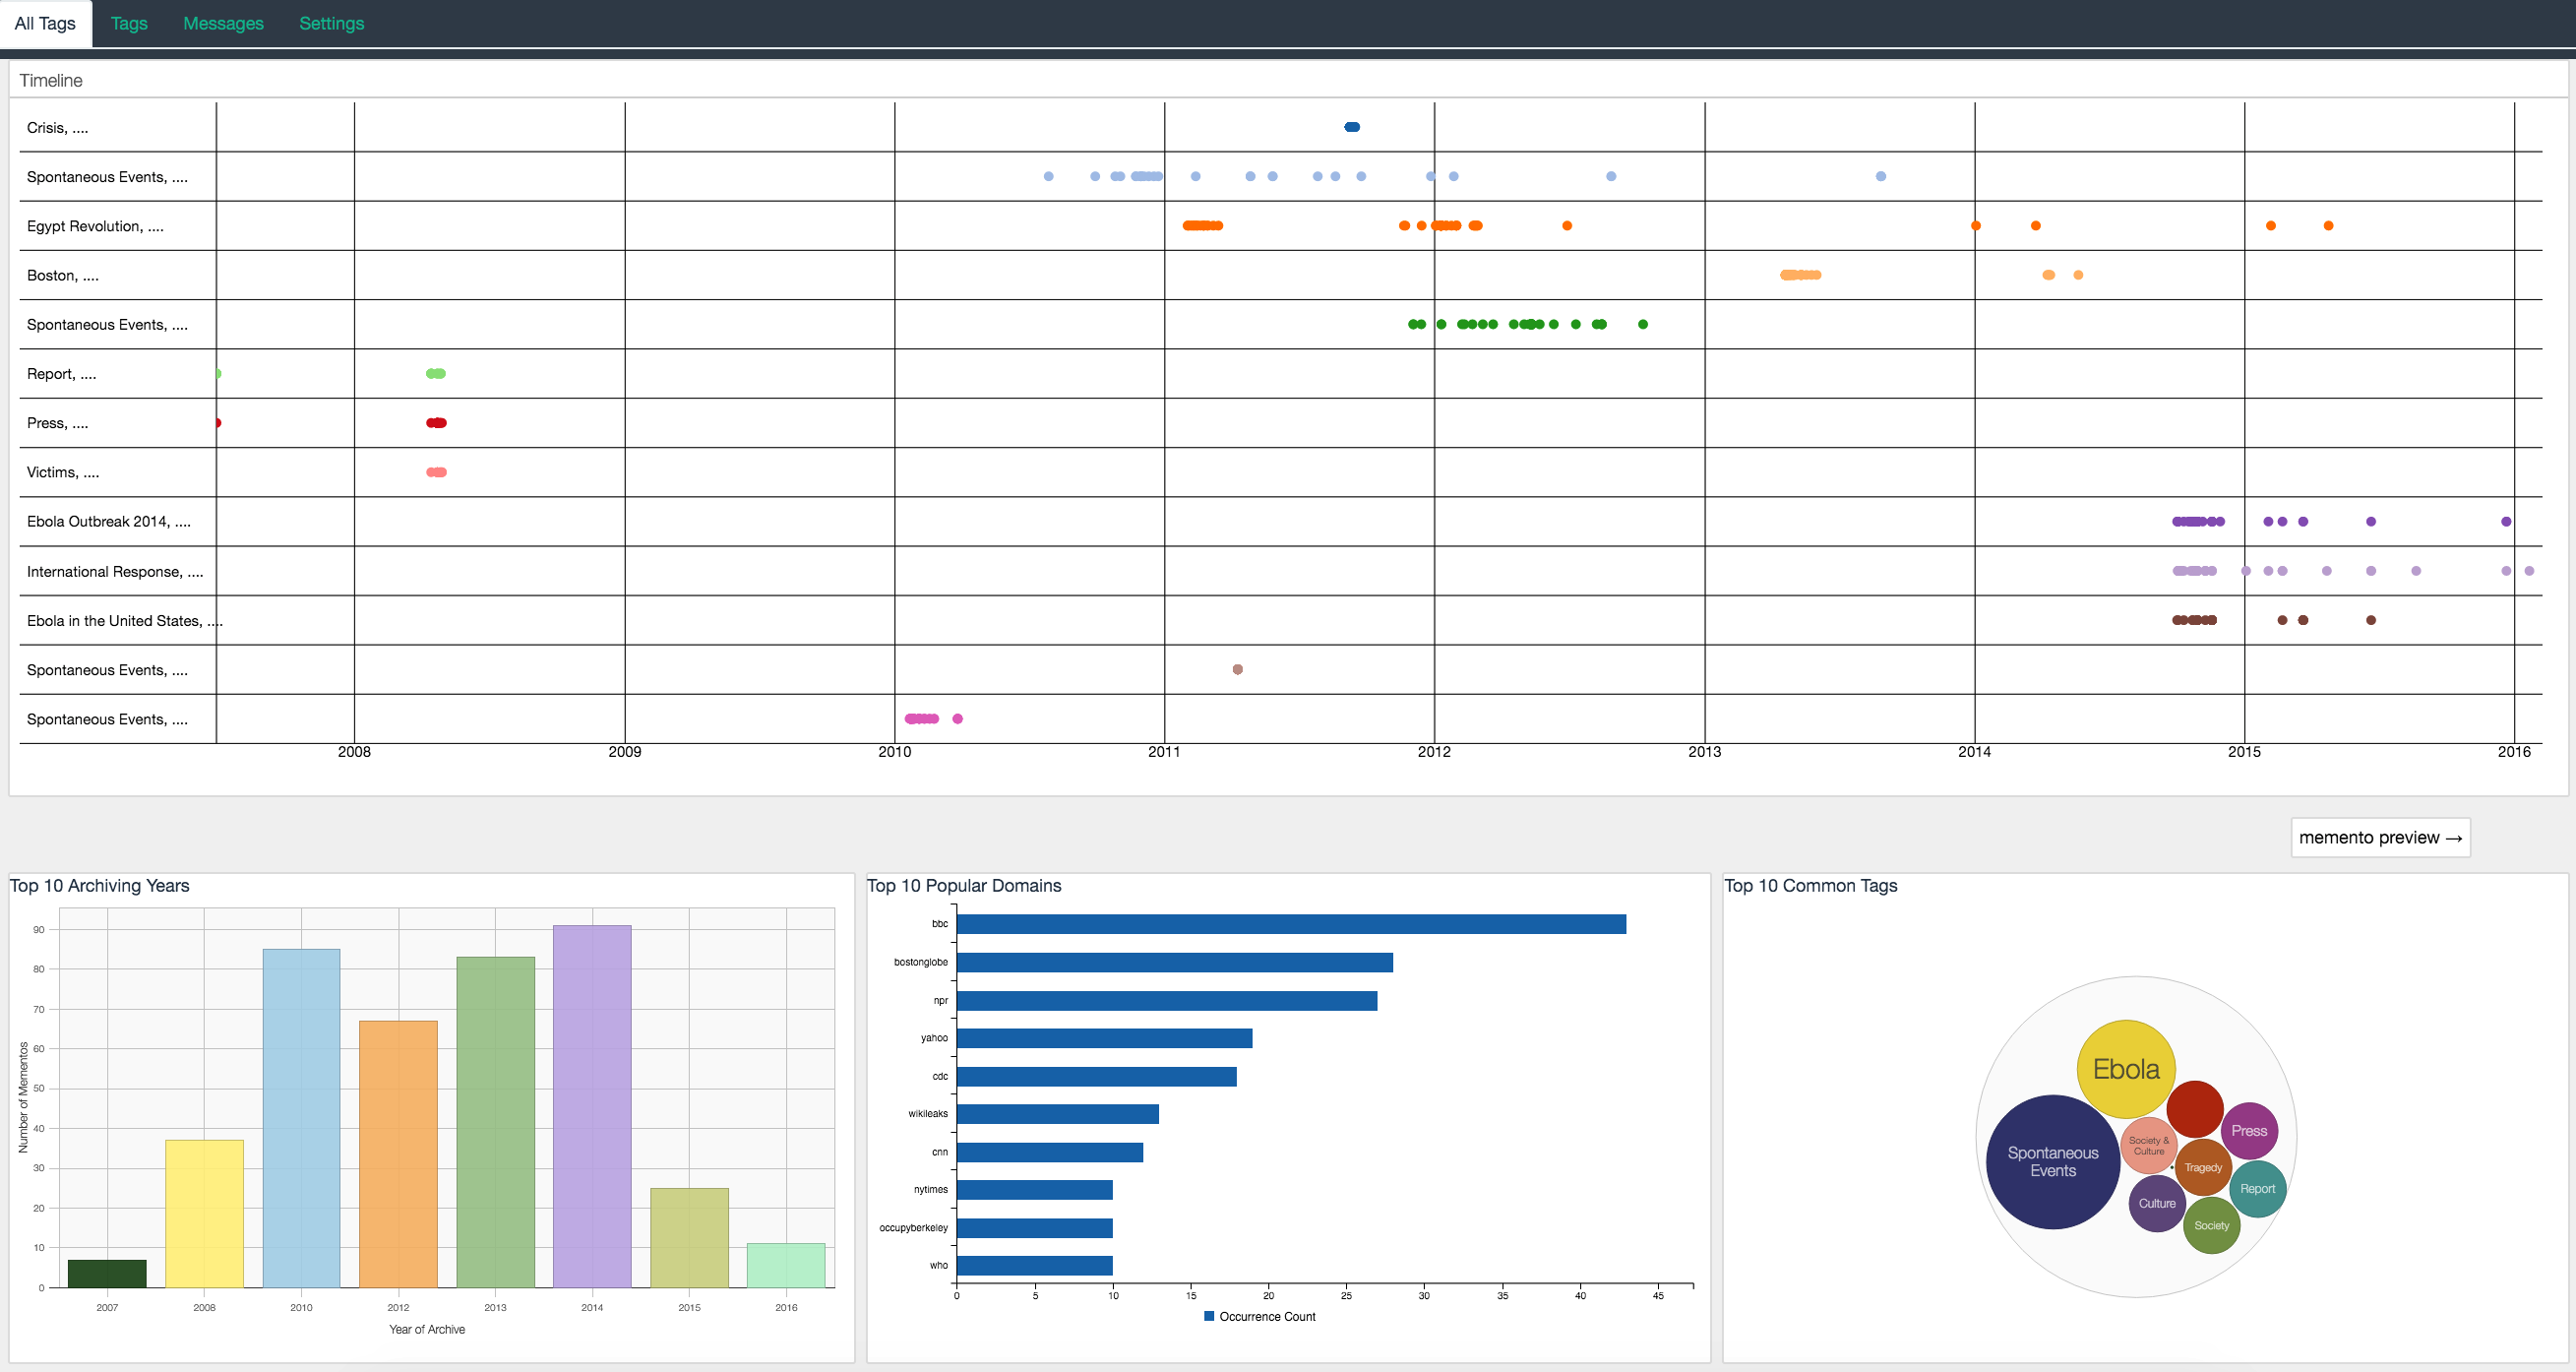
\includegraphics[scale=0.1]{Figure1}
\caption{Web Archive Visualizer}
\label{fig:mesh1}
\end{figure}

In our current solution, Web Archive Visualizer, we propose an approach that addresses those problems. The idea behind uur solution, is that contextual information created during time of archive, such as the name and keywords associated with a resource, can create a set of useful characteristics about the data. Using this additional information, we are not only able to relate sub sections of an archive, but also limit both the amount and the types of resources shown. While the cost of going through an archival process is substanitially higher, the increase in overall understading far outweighs its limitations. Web Archive Visualizer can be seen in Fig. 1, where we system is seperated into multiple views denoting particular points of interest. \par

\begin{figure*}
\centering
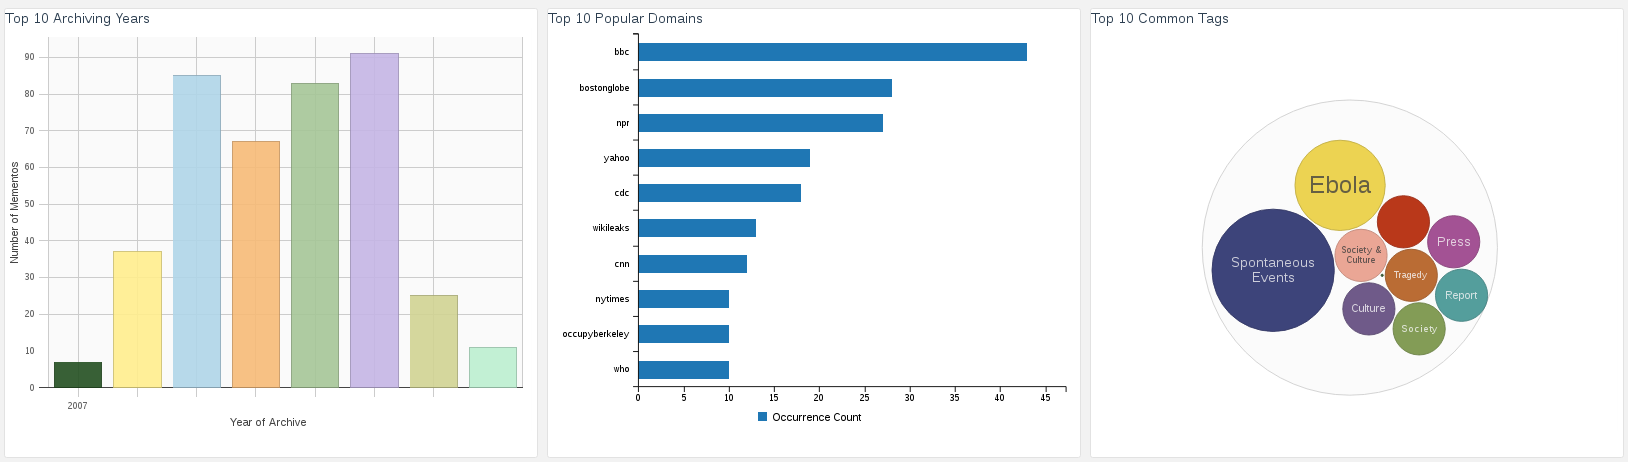
\includegraphics[width=\textwidth]{Figure3a}
\caption{This figure shows the general idioms that apply to the entire collection.}
\label{fig:mesh2}
\end{figure*}

\section{Related Work}
The vast majority of current and previous works of web archive visualizations places a heavy focus on their evolution. Dating back to 2005, the developers behind WebRelievo \cite{toyoda2005system} propose a visualization to monitor the change of resources within a web archive over a particular period. Aside from a known archival date, the goal of the system aims to identify relationships between different web resources without any contextual data. In another words, they aim to see the interconnecting of the web and how it differs over a span of years, without taking any additional characteristics from the original archivers. Even though there is a lack of contextual data, WebRelievo is a promotes a good step towards relationship identification of resources within collections, regardless of the collection size. \par

Older works, such as those in \cite{toyoda2003extracting}, show relationships between resources located within similar communities. In this context, communities are clusters that all relate to a particular topic. While this approach also uses only temporal attributes of the archival process, the authors show the importance of identifying points of interest within a web archive. The general idea of this work directly supports ours, in which we leverage relationship identification of like meta data, i.e. tags and temporal attributes, to help classify and discover potential areas of interest. \par


\section{Design}
The realestate of the viewers attention is split into multiple views of interest, as seen in Figure \ref{fig:mesh1}. In the top portion of the screen, referred to as the main content, users are given the ability to view specific characteristics of all data within the archive. The main content is followed by arrows for navigation between different specific views. The text of the navigation links dynamically changes to alert the user about the next and previous idoms in line. TODO:: this sounds stupid. \par

On the contrary, the bottom portion outlines multiple views for more general characteristics that can summarize the entire collection. We refer to this section as the complementary content. Note, this split of interest between these two sections is important, as it gives users more control on the amount of data that they see at once. In essence, this is a strategically enforced measure to ensure cognitive memory does not become overloaded. Unlike the main content, views within the complemeplentary content are always shown, as a proactive measure enabling comparison of data between the more specific content and the overall message sent my the web archive collection. \par

To make the boundry between main and complementary contents more clear to the user, we seperate generated visualizations by the area of categorical influence. This causes resource speicfic views to fall into several categories, including: timeline of resource archives, thumbnail views of mementos, resource clusers, and keyword groupings. They are granular enough to ensure that the targeted audiance can fork out and create relationships of the low level details surrouding their data. On the contrary, idioms showing general characterisicts primarily focus on the higher level summaries, such as outlining the most active archiving years, popular domains, and the most common tags. \par 

\begin{figure*}
\centering
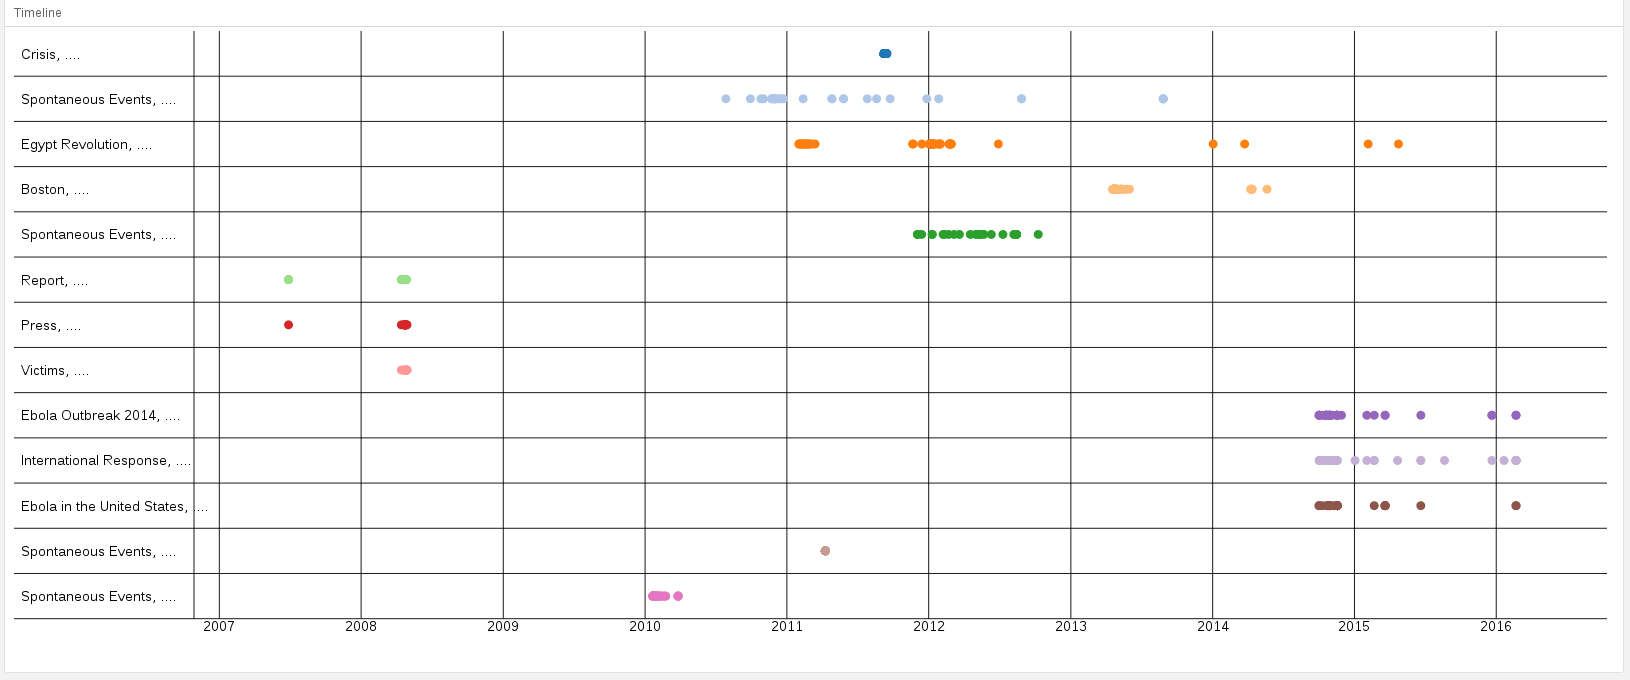
\includegraphics[width=\textwidth]{Figure4}
\caption{Timespan chart showing archives associated with particular tags}
\label{fig:mesh3}
\end{figure*}

\subsection{Resource specific idioms}
One of the primary areas of focus, alike most recent work, is time. Knowing when a particular resource was archived, is the first step in identifying differences over time and drawing stories as they evolve (TODO:: YASMIN). For this reason, Web Archive Visualizer places primary focus on TODO:: CHARTNAME, as seen in Figure \ref{fig:mesh3}. The purpose of this idiom is to let users view keywords associated with archived resources, over time. Aside from the obvious, keyword dominance over time, this chart also allows us to see the levels of activity as the collection years grow.

\subsection{General idioms}
Figure \ref{fig:mesh2} shows three different general views. The left most view, memento activy over a set of years, denotes the number of archives present for a particular resource in some time. Understanding the most active years has many advantages to archivers and general users exploring the collection. First, it allows them to conceptually visualize what periods of activity are responsible for the peaks within the collection. If the collection has a specific context, such as an archive consisting of hurricane events, particular years could outline the most influential years. The same is also true for identifying trends or outliers in data, where perticular years might show a steady incline, decline, or abnormal levels of mementos collected. \par

Most popular domains, middle view in Figure \ref{fig:mesh2}, shows where most of the resources are being collected from. This is especially important to know when understanding domain reliance or influence of content of the web archive. Alike the idiom denoting years, understanding domain dominance can also help outline the skewedness and bias within our collections. This is especially helpful, when the arciving team is collecting mementos relating to one particular category from a limtless scope of domains. \par

The last view in Figure \ref{fig:mesh2} shows the most popular tags, whose occourance count is represented in an increased size. Once a tag dominates the others, we can gain more contextual awareness regarding our data. This can help us answer questions like: are we focusing on archiving particular areas? are there particular keywords associated with our collection subset? Having this general view is also especially helpful when attempting to combine it to the specific charts outlined above. Since it is easy to see the number of times a keyword occoured in our collection, TODO: CHARTNAME, can let us see how words of interest compare to those that are most popular. \par

\subsection{What Why How Framework}
TODO::

\section{Evaluation}

To perform our evaluation, we ran two different expeirments. The first was a metric to see associated perfomrance with the following system. Shown in figure 5.

\begin{figure}[b]
\centering
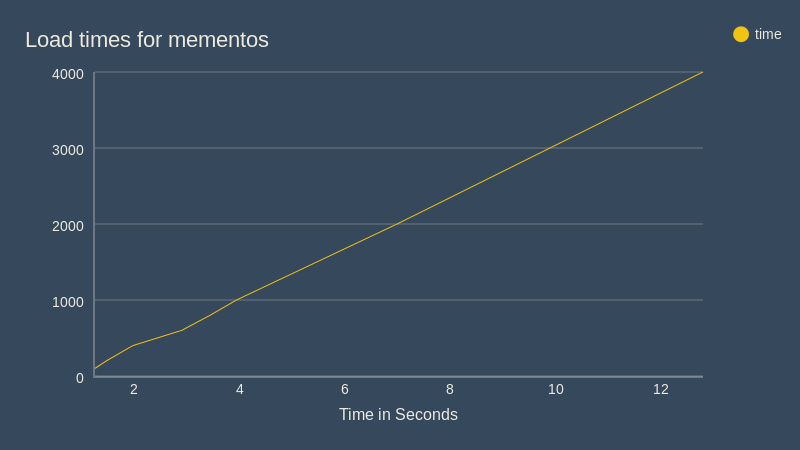
\includegraphics[scale=0.2]{Figure5}
\caption{Duration of loading memenots over time}
\label{fig:mesh4}
\end{figure}

100,1.25
200,1.47
400,1.97
600,2.90
800,3.44
1000,3.94
2000,6.99
4000,12.80


\section{Conclusion}
The conclusion goes here.

\section{Final Thoughts}



\ifCLASSOPTIONcompsoc
  % The Computer Society usually uses the plural form
  \section*{Acknowledgments}
\else
  % regular IEEE prefers the singular form
  \section*{Acknowledgment}
\fi


The authors would like to thank...


% Can use something like this to put references on a page
% by themselves when using endfloat and the captionsoff option.
\ifCLASSOPTIONcaptionsoff
  \newpage
\fi



% trigger a \newpage just before the given reference
% number - used to balance the columns on the last page
% adjust value as needed - may need to be readjusted if
% the document is modified later
%\IEEEtriggeratref{8}
% The "triggered" command can be changed if desired:
%\IEEEtriggercmd{\enlargethispage{-5in}}

% references section
\bibliography{mybib}{}

% can use a bibliography generated by BibTeX as a .bbl file
% BibTeX documentation can be easily obtained at:
% http://mirror.ctan.org/biblio/bibtex/contrib/doc/
% The IEEEtran BibTeX style support page is at:
% http://www.michaelshell.org/tex/ieeetran/bibtex/
\bibliographystyle{IEEEtran}
% argument is your BibTeX string definitions and bibliography database(s)
%\bibliography{IEEEabrv,../bib/paper}
%
% <OR> manually copy in the resultant .bbl file
% set second argument of \begin to the number of references
% (used to reserve space for the reference number labels box)

\end{document}


